\section{Mcp-Executor-Einheit}
\label{kap:McpExecutorEinheitMain}
Die Mcp-Executor-Einheit definiert ein Gerät, welches Beschleunigungsdaten über SPI an ein Master-Gerät schickt, sobald es eingeschaltet wird.
\newline
Für diese Funktionalität werden die in Kapitel \ref{kap:McpExecutorVerwendeteKomponenten} beschriebenen Komponenten verwendet, welche wie in Abbildung \ref{fig:Mcp2515EinheitZusammenspiel} dargestellt entsprechend verknüpft sind.

	\begin{figure}[H]
		\centering
		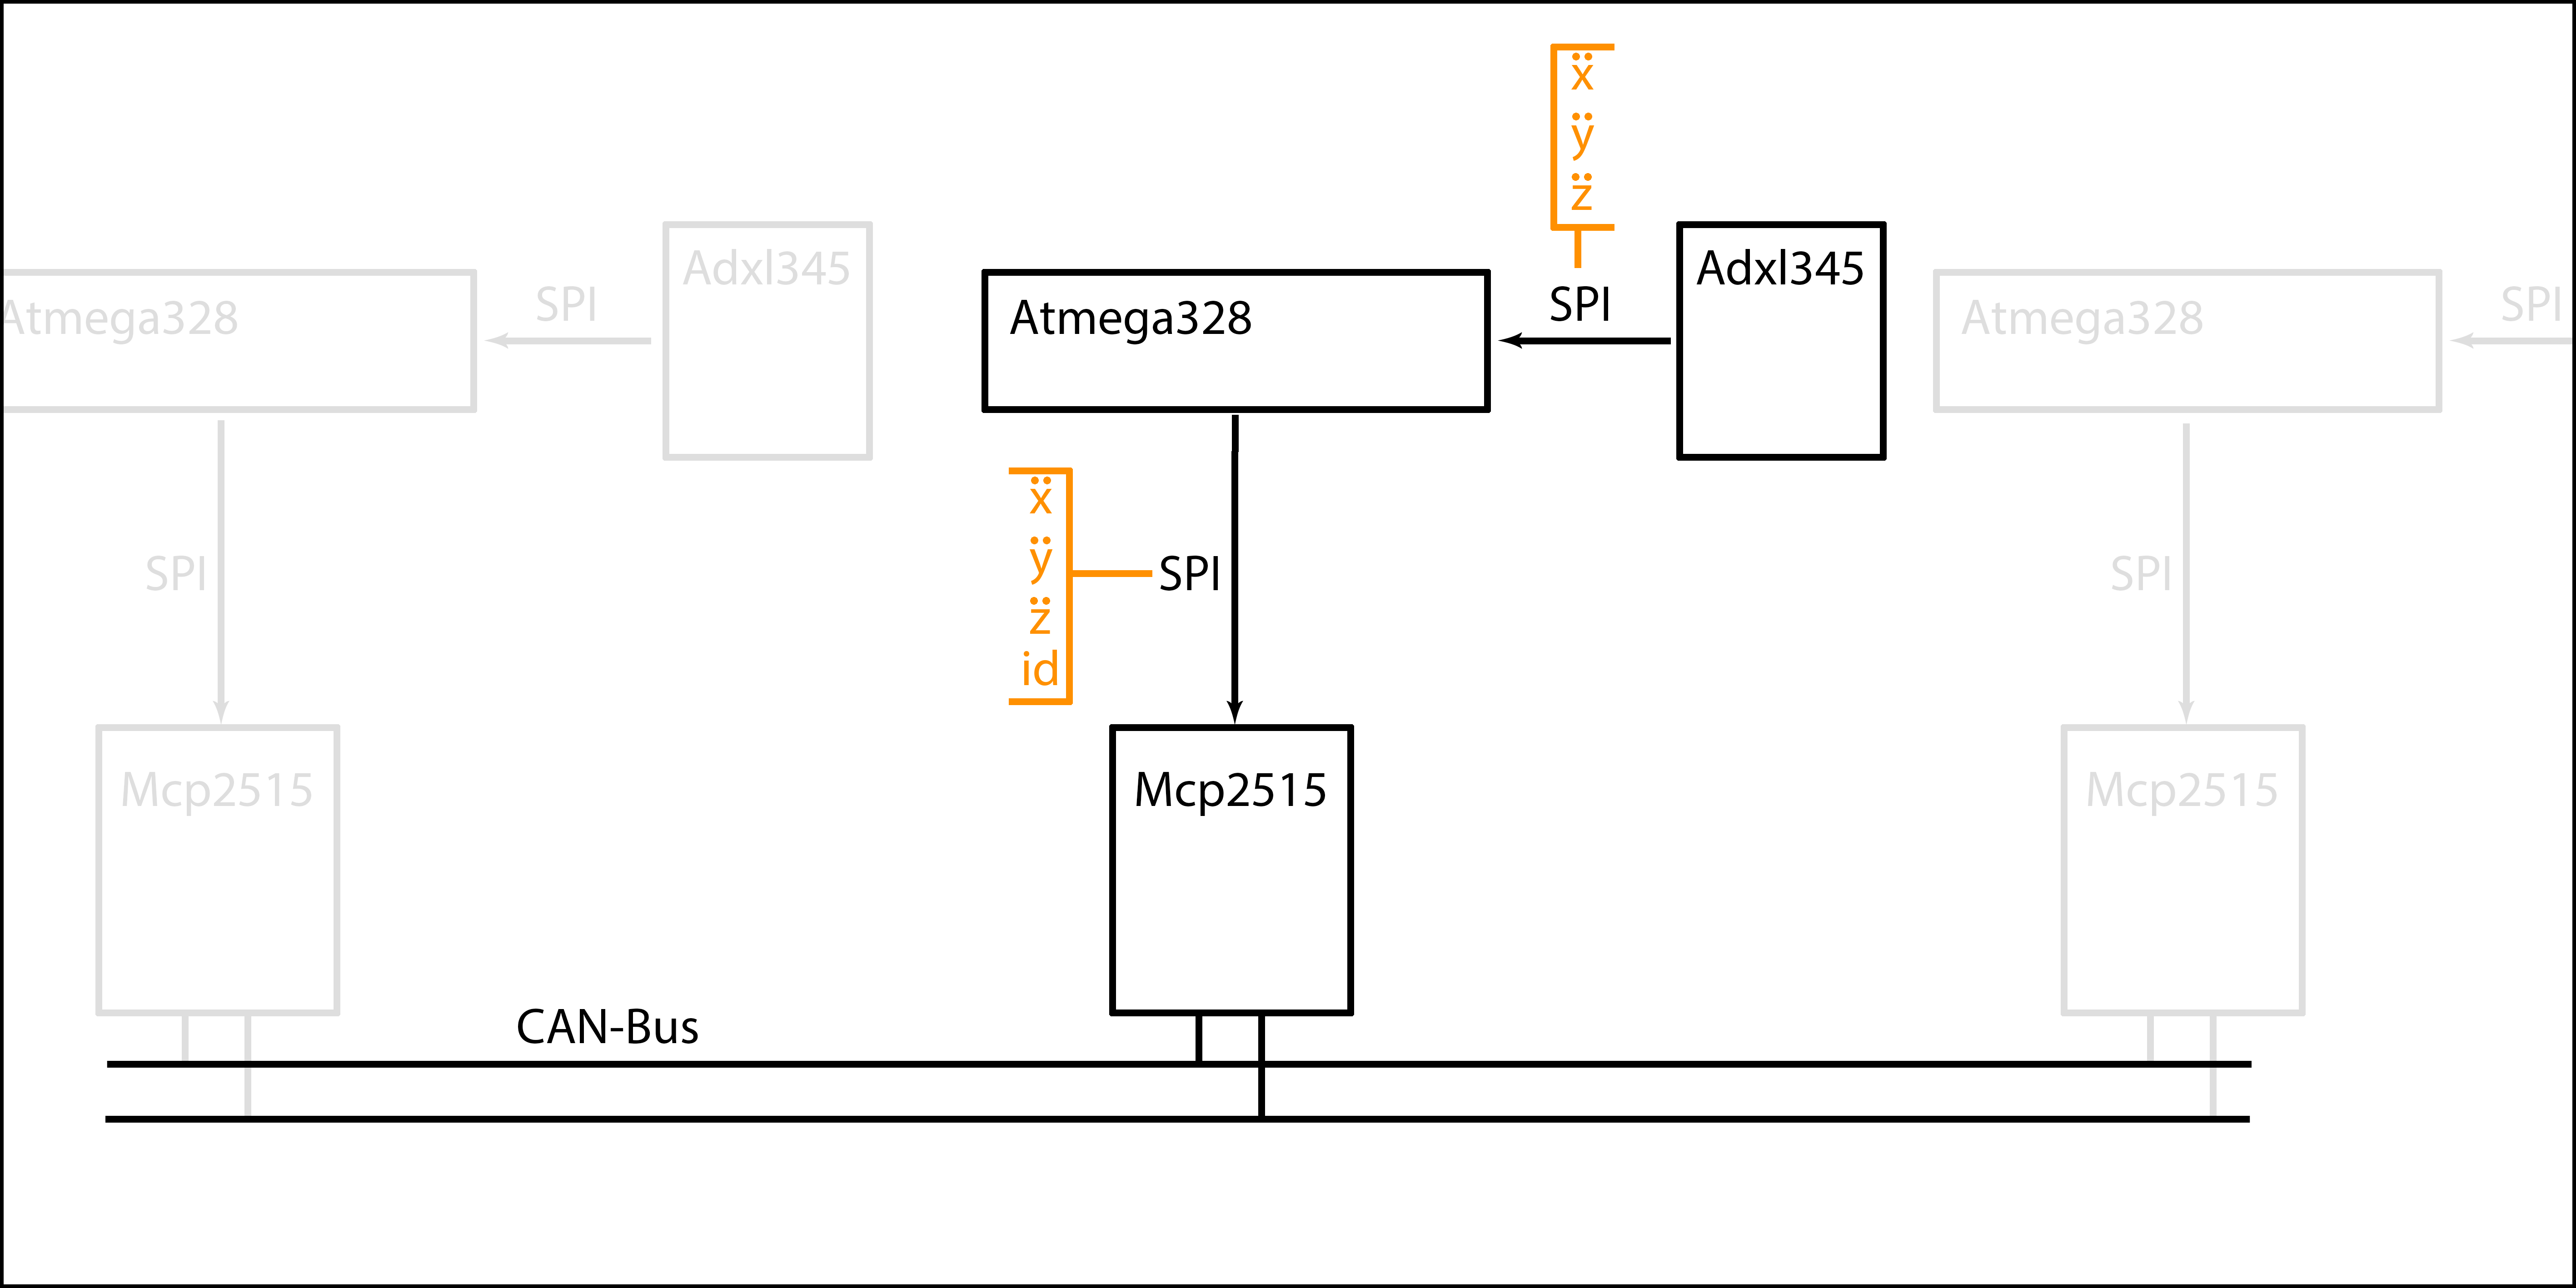
\includegraphics[width=1.0\linewidth]{Bilder/Mcp2515EinheitZusammenspiel}
		\caption[Zusammenspiel der Komponenten Mcp-Executor-Einheit]{Zusammenspiel der Komponenten Mcp-Executor-Einheit}
		\label{fig:Mcp2515EinheitZusammenspiel}
	\end{figure}
	
Der Microcontroller Atmega328 ließt von dem Beschleunigungssensor Adxl über die Schnittstelle SPI Sensordaten aus und gibt diese (ebenfalls über SPI) an den Mcp2515 weiter. Dieser schiebt die Daten auf den CAN-Bus.
	
\subsection{Verwendete Komponenten}
\label{kap:McpExecutorVerwendeteKomponenten}
Für eine Einheit werden verschiedene Hardware-Komponenten verwendet, deren Wahl vor allem hinsichtlich des Kostenaufwandes erfolgte. Auch die Bauteilgröße ist ein entscheidender Faktor, da die Einheiten möglichst nicht störend sein sollen.

\begin{itemize}
	\item \textbf{Mcp2515}
	
	Der Mcp2515 beschreibt an sich den Chip, welcher auf der, in Abbildung \ref{fig:Mcp2515} dargestellten, Platine verbaut ist. Dieser Name wird jedoch für den gesamten Chip verwendet.
	\newline
	Die Funktion des Mcp2515 besteht darin Daten über die Schnittstelle SPI zu empfangen und über einen CAN-Bus zu versendet. Die Steuerung des Chips (z.B. Beschreiben eines Sende-Buffers) erfolgt dabei mit entsprechenden Kommandos über SPI. Das Konvertieren in L-, H-Pegel erfolgt komplett automatisch.
	
	\begin{figure}[H]
		\centering
		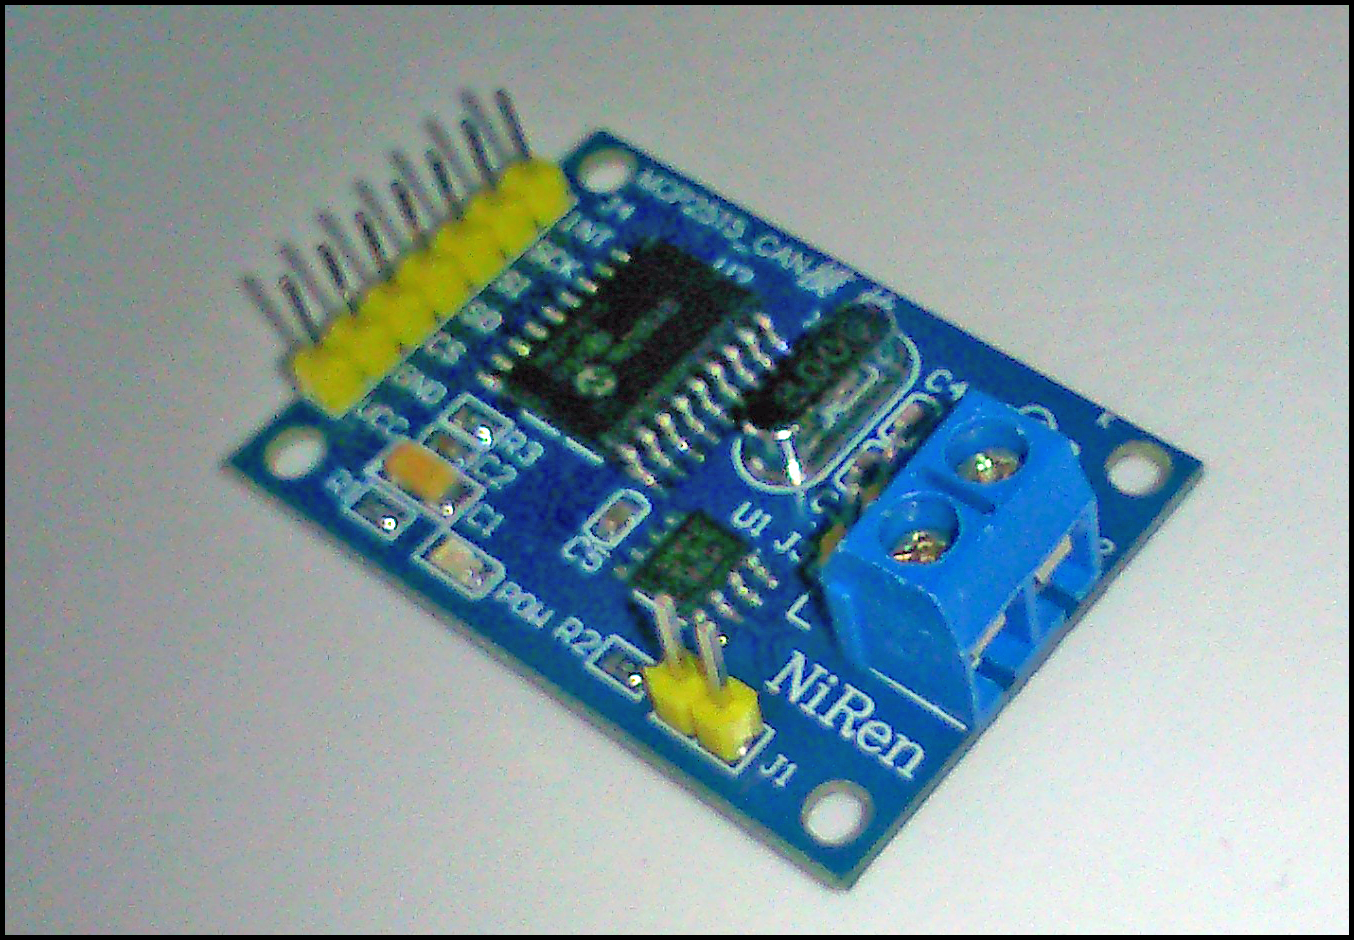
\includegraphics[width=0.4\linewidth]{Bilder/Mcp2515}
		\caption[Mcp2515]{Mcp2515}
		\label{fig:Mcp2515}
	\end{figure}
	
	\item \textbf{Adxl345}
	
	Bei dem Adxl345 handelt es sich um einen 3-Achsen Beschleunigungssensor (s. Abbildung \ref{fig:Adxl345}), dessen Messwerte über SPI in verschiedenen Genauigkeiten ausgelesen werden können.
	Der Chip besitzt eine äußerst geringe Leistungsaufnahme und ist kompatk in seiner Bauform.
		
	\begin{figure}[H]
		\centering
		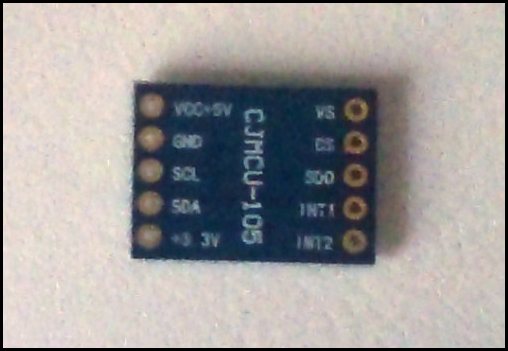
\includegraphics[width=0.4\linewidth]{Bilder/Adxl345}
		\caption[Adxl345]{Adxl345}
		\label{fig:Adxl345}
	\end{figure}
	
	\item \textbf{Atmega328}
	
	Der Microcontroller Atmega328 ist u.A. in dem Arduino-Board verbaut. Es ist ein kostenfünstiger Allrounder, welcher hauptsächlich wegen seiner großen Verbreitung gewählt wurde.
	Der Chip (s. Abbildung \ref{fig:Atmega328}) besitzt eine SPI-Schnittstelle und diverse I/O's, weshalb die Projektanforderungen vollständig erfüllt werden.
	\newline
	Es exisiteren zwei verschiedene Versionen des MCU's, von denen die Atmega328-P Variante für eine geringe Leistungsaufnahme konzipiert ist. 
	
	\begin{figure}[H]
		\centering
		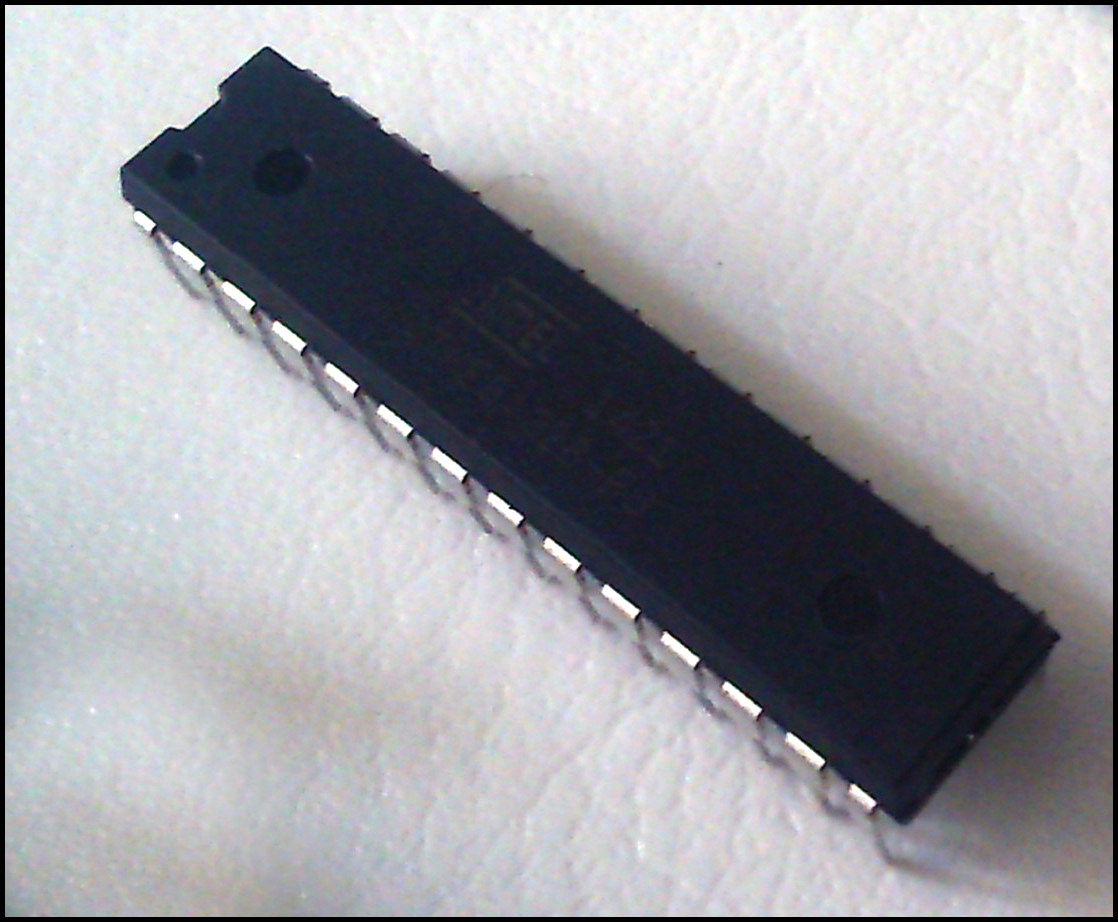
\includegraphics[width=0.4\linewidth]{Bilder/Atmega328}
		\caption[Atmega328]{Atmega328}
		\label{fig:Atmega328}
	\end{figure}
	
	\item \textbf{Oscillator und Kondensator}
	
	Der Atmega328 benötigt einen externen Taktgeber, welcher mit einem 16Mhz Quarz und entsprechenden Kondensatoren gewählt wird (s. Abbildung \ref{fig:Oscillator}).
	
	\begin{figure}[H]
		\centering
		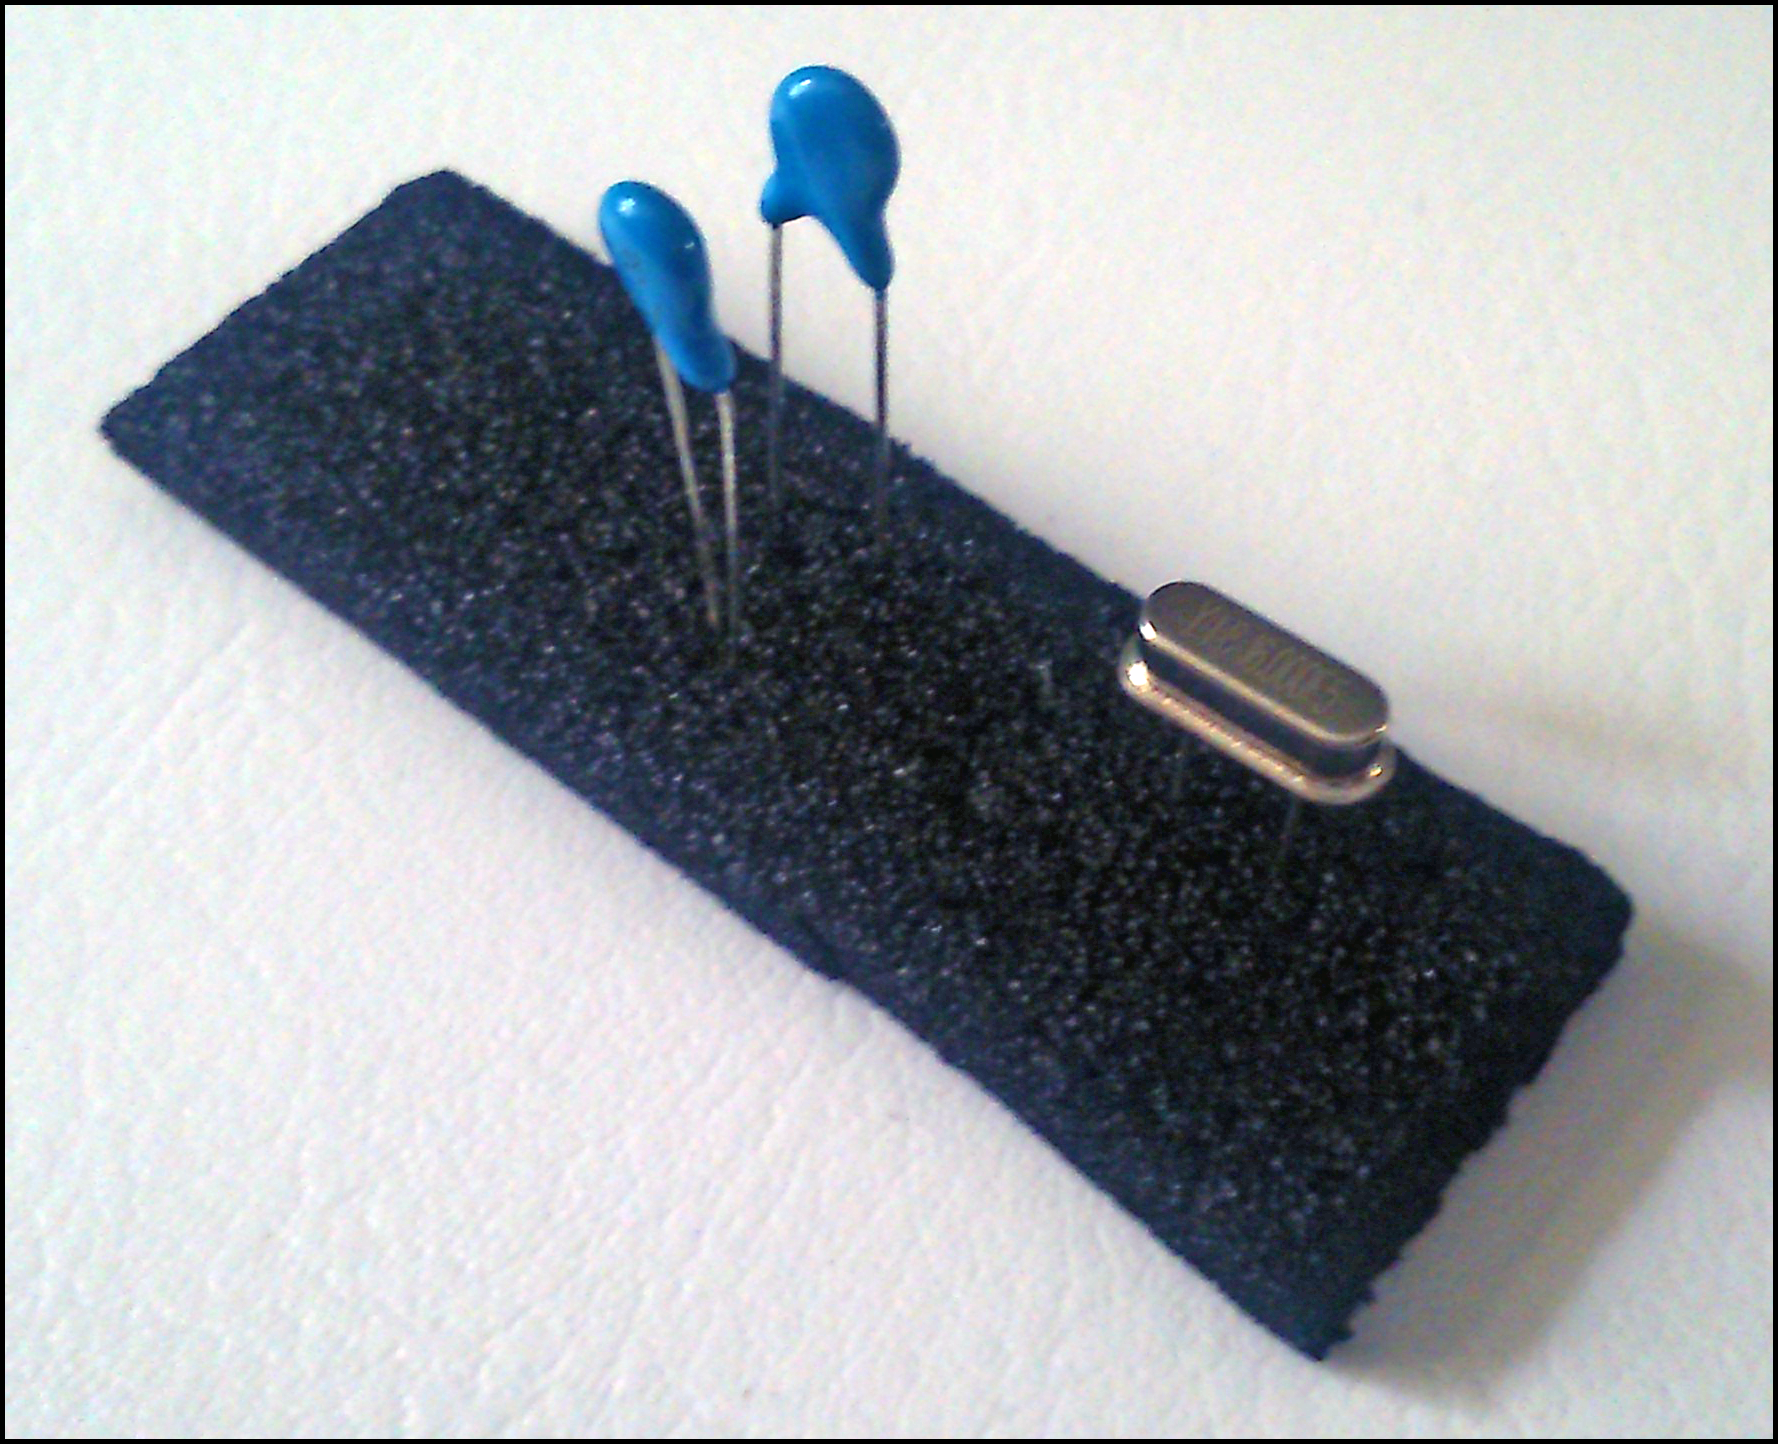
\includegraphics[width=0.4\linewidth]{Bilder/Oscillator}
		\caption[Oscillator]{Oscillator}
		\label{fig:Oscillator}
	\end{figure}
		
\end{itemize}
\subsection{Testversion}
\label{kap:McpExecutorTestversion}
Um die Funktionen der Chips zu verstehen und beherrschen zu können erfolgt der Aufbau einer Einheit auf einem Entwicklungsboard (Whiteboard). Dieser Aufbau beinhaltet alles, was für eine Einheit vorgesehen ist, d.h. einen Atmega328 (mit externem Taktgeber), einen Adxl345 und einen Mcp2515. Mit entsprechender Verdrahtung (s. Schaltbild \ref{fig:SchaltbildEinheit}) und der Entwicklung eines Programms, welches auf der MCU aktiv ist, lassen sich die Sensorwerte über einen CAN-Bus auslesen. Die Sensor-ID muss programmatisch auf der MCU definiert werden. 

\begin{figure}[H]
	\centering
	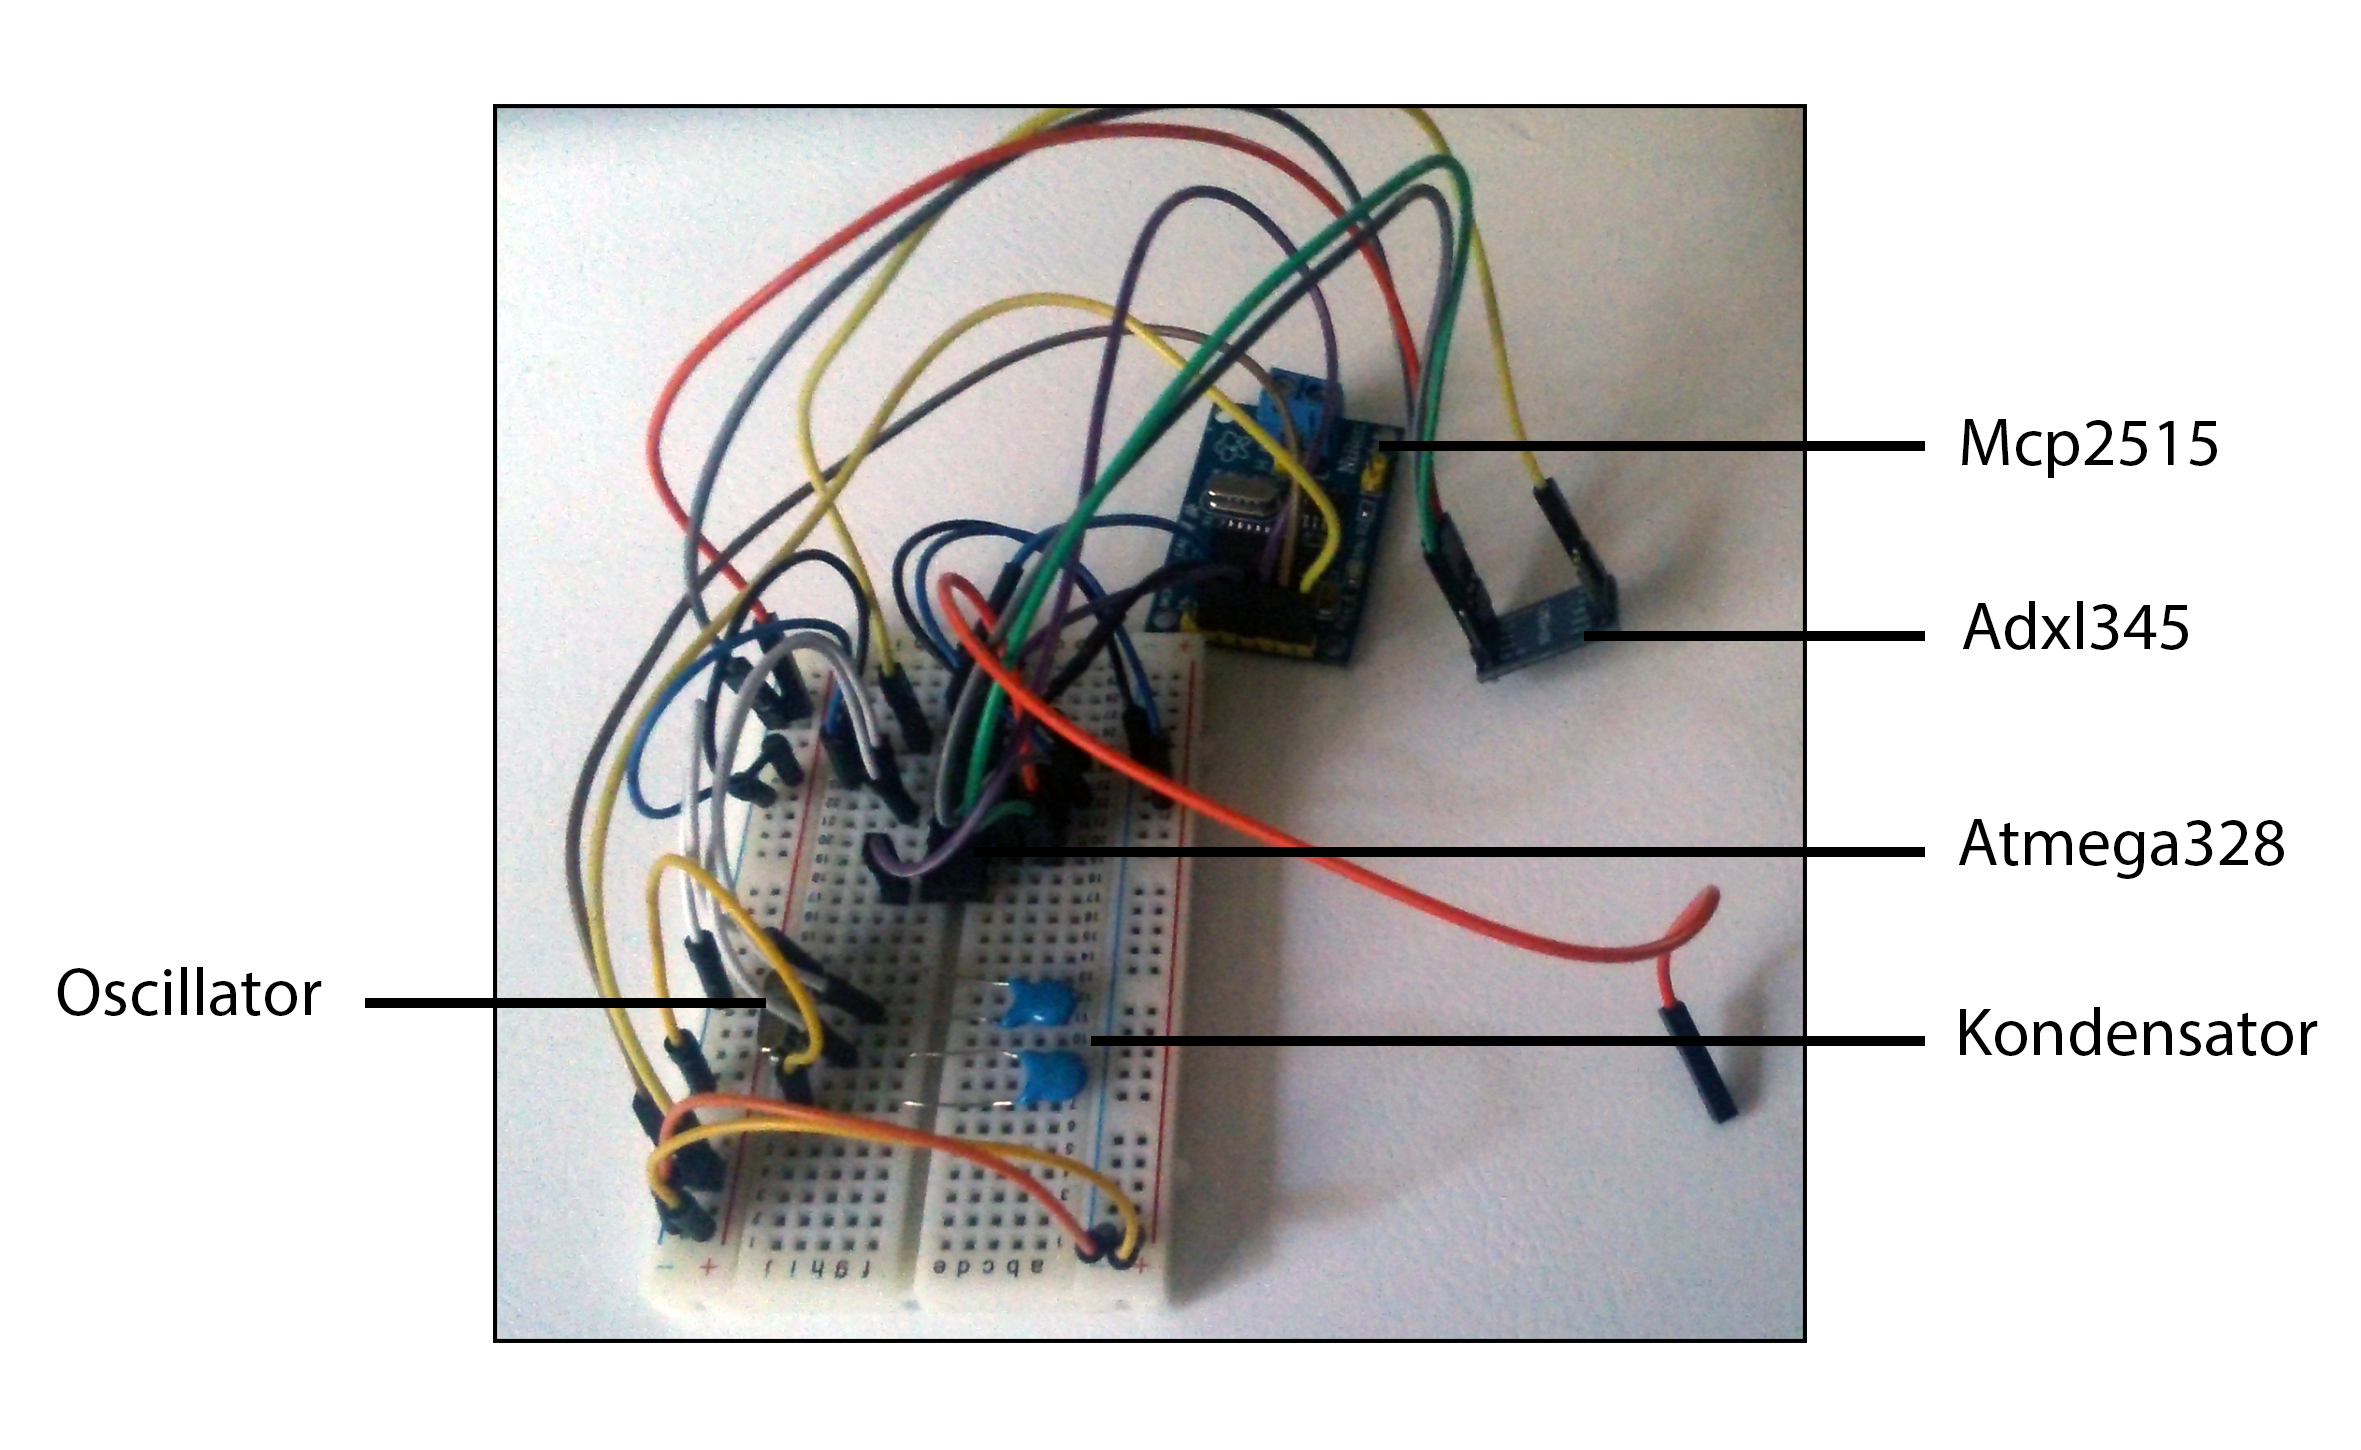
\includegraphics[width=0.9\linewidth]{Bilder/McpExecutorTest}
	\caption[Testversion einer Mcp-Executor-Einheit]{Testversion einer Mcp-Executor-Einheit}
	\label{fig:McpExecutorTest}
\end{figure}

Mit zwei solcher Testaufbauten wurde das Aufnehmen von Sensorwerten validiert.
\subsection{Beta version}
\label{kap:McpExecutorBetaversion}
Für die Betaversion der Mcp-Executor-Einheit werden alle Komponenten in ein Gehäuse integriert (s. Abbildung \ref{fig:McpExecutorBeta}), welches gerade so groß ist, dass es beim Tragen am Körper möglichst nicht stört und einfach befestigt werden kann. Für das Integrieren werden zusätliche Platinen angefertigt.
\newline
Aufgrund des Feststellens verschiedener negativer Aspekte während der Entstehung der EInheiten existieren mehrere Beta-Versionen.

\begin{figure}[H]
	\centering
	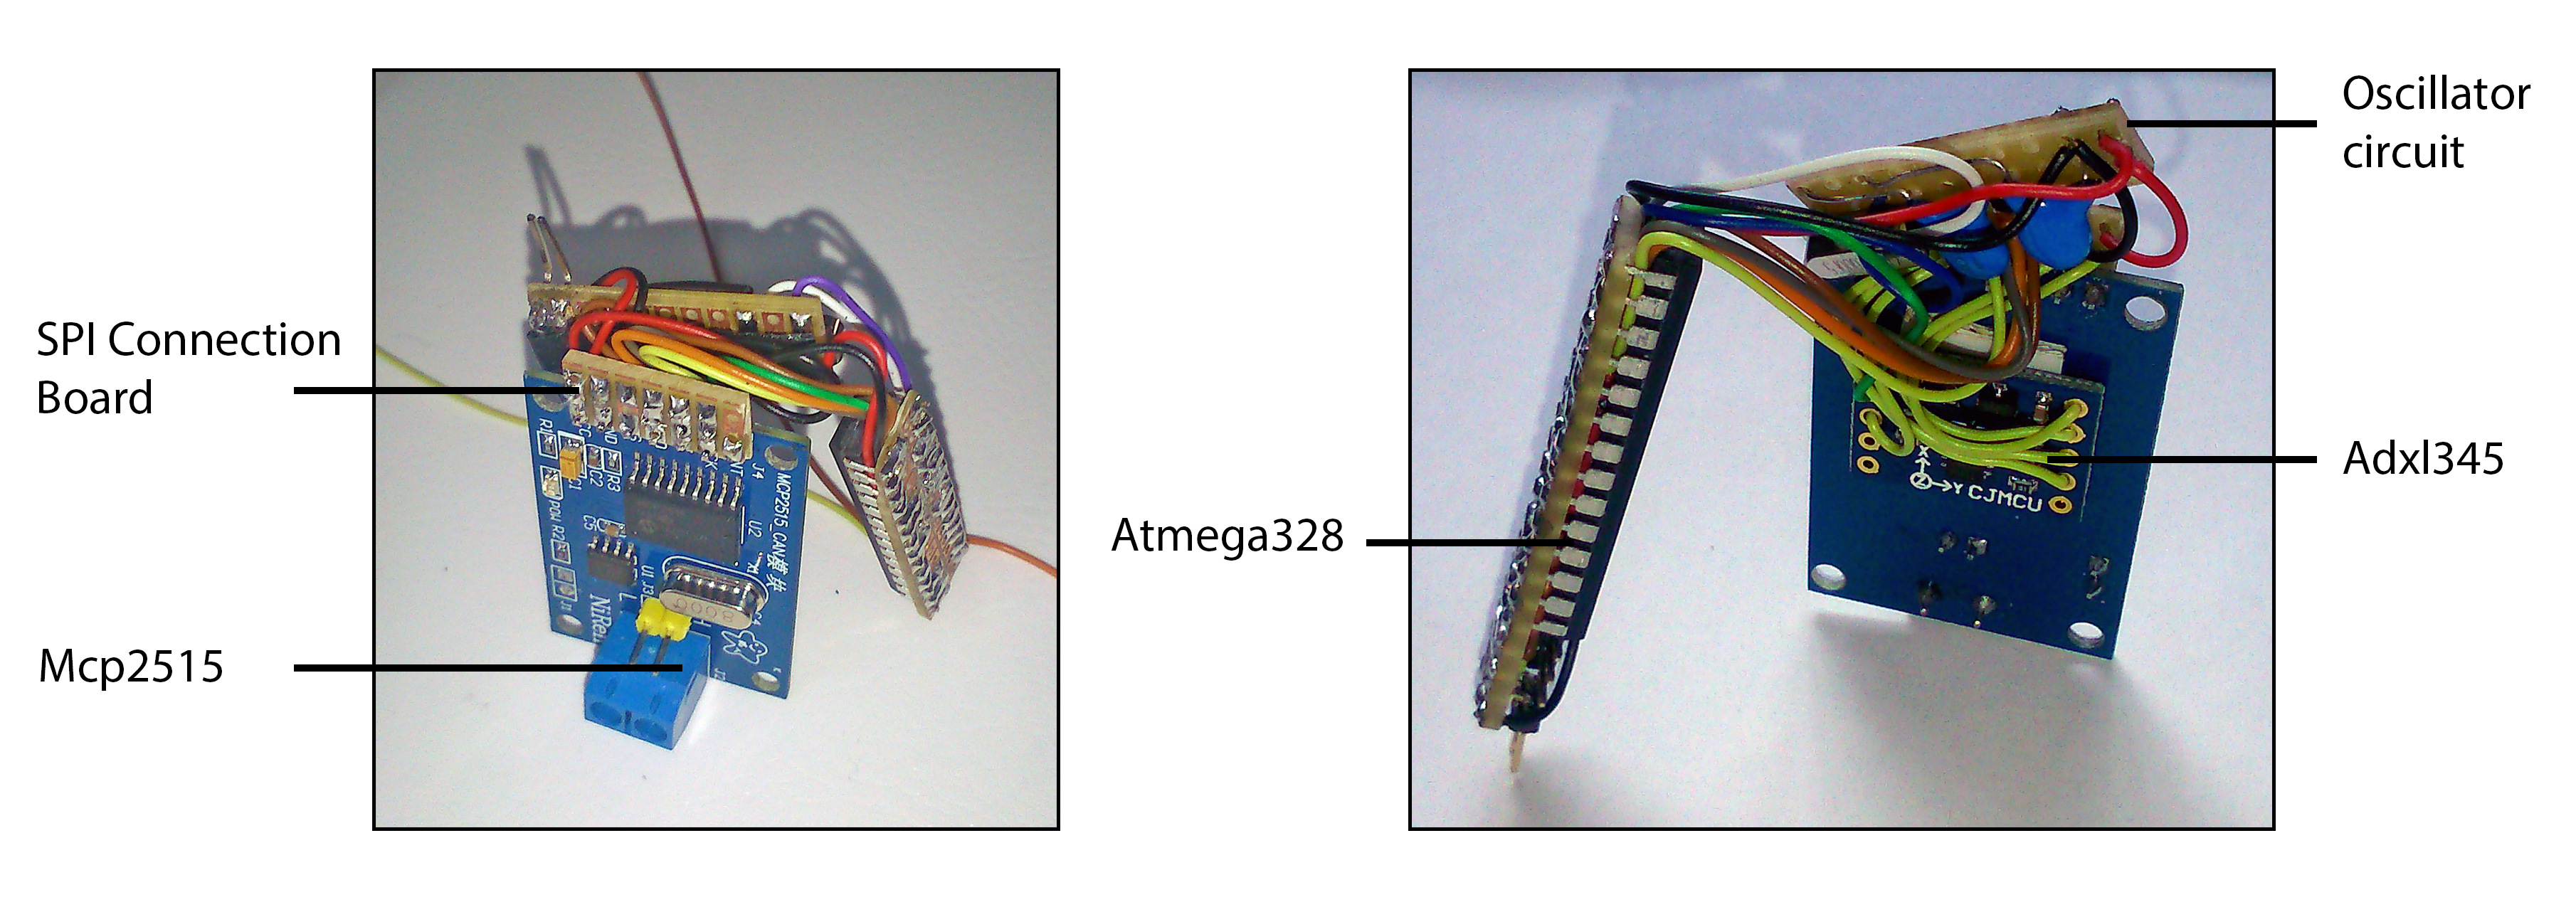
\includegraphics[width=1.0\linewidth]{Bilder/McpExecutor_BetaDetail}
	\caption[Betaversion einer Mcp-Executor-Einheit]{Betaversion einer Mcp-Executor-Einheit}
	\label{fig:McpExecutorBeta}
\end{figure}

Die Befestigung der Einheit am Körper erfolgt anhand eines Positioniergurtes. Dieser besteht in der ersten Beta-Version aus zwei und in der zweiten Version aus einem Klettverschluss, die an dem Abdeckblech der Einheit befestigt sind. Durch ein entsprechendes Gegenstück des Klettverschlusses auf der Rückseite des Abdeckblechs ist der notwendig Halt gegeben.
%
% BILD KLETTVERSCHLUSS
%
\begin{figure}[H]
	\centering
	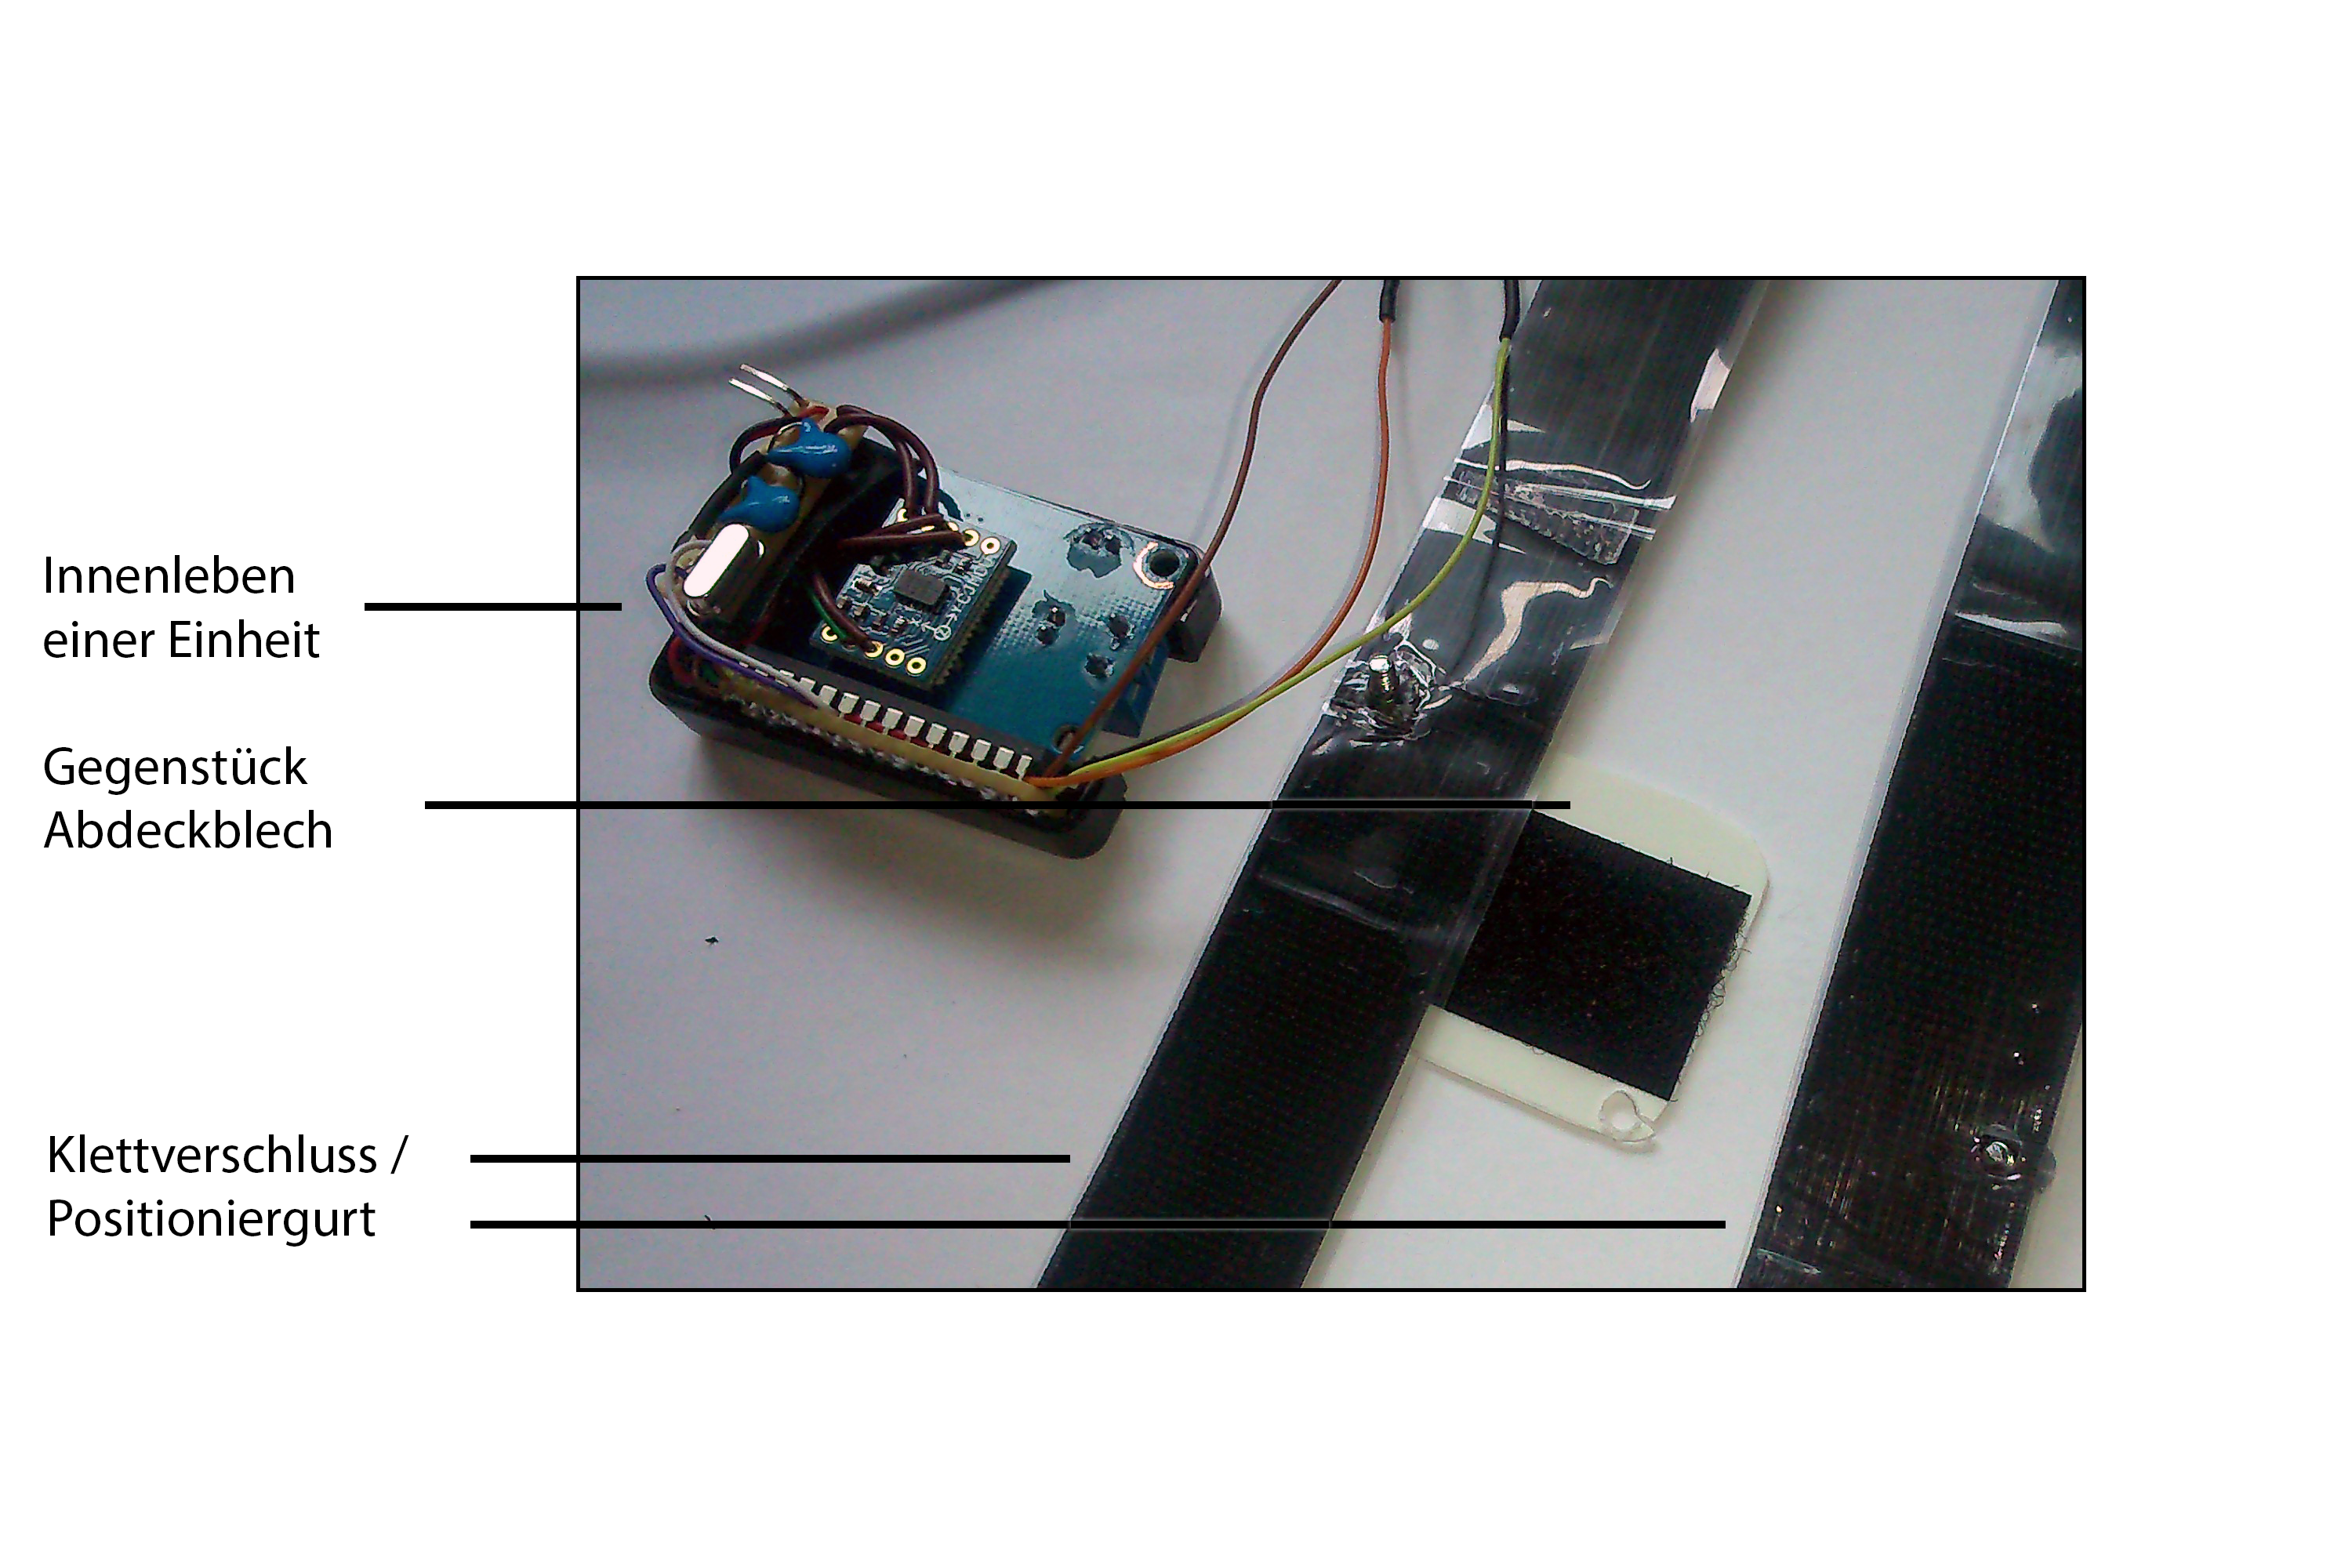
\includegraphics[width=1.0\linewidth]{Bilder/McpExecutor2515Klettverschluss}
	\caption[Betaversion einer Mcp-Executor-Einheit - Klettverschluss]{Betaversion einer Mcp-Executor-Einheit - Klettverschluss}
	\label{fig:McpExecutorBetaKlettverschluss}
\end{figure}

An dem Anzug sind ebenfalls entsprechende Gegenstücke des Klettverschlusses angebracht, sodass die Einheiten während der Bewegung nicht verrutschen. 


\subsection{Pre-Release version}
\label{kap:McpExecutorPreReleaseversion}
Bei der Pre-Realease-Version der Mcp-Executor-Einheit wird die Beta-Version zunächst bewertet und alle negativen Aspekte aufgezeigt und möglcihe Lösungen erarbeitet. Die zu verbessernden Punkte sind in Tabelle \ref{tab:McpExecutorEinheitNegAspekte} aufgelistet:

% INSERT TABLE WITH NEGATIVE ASPECTS
\begin{table}[H]
	\caption{Optimierung der Beta-Version}\label{tab:McpExecutorEinheitNegAspekte}
	\centering
	\begin{tabular}{|p{5cm}|p{5cm}|}
		\hline
		\textbf{Negativer Aspekt} & \textbf{Lösung} \\
		\hline
		Spalt zwischen Abdeckblech u. Gehäuse & Höhe um 2mm verringern \\
		\hline
		Gehäuse ist nach außen gebogen & Breite um 1mm verringern \\
		\hline
		Rxd, Txd, Reset Leitungen nicht befestigt & ANschlüsse als Stecker ausführen \\
		\hline
		VCC und GND nicht auf gleicher Seite wie Bus-Anschluss & Anschlüsse seitlich aus Gehäuse herausführen \\
		\hline
		Osc1, Osc2 Leitungen sind eingeklemmt & Leitungen seitlich aus MCU herausführen \\
		\hline
		Kunststoffabdeckung biegt sich durch & AL-Platte verwenden \\
		\hline
		VCC, GND Anschluss nicht fixiert & Platine verlängern und in Gehäuse klemmen \\
		\hline
		Platinen unzureichend in Richtung des Abdeckblechs fixiert & Puffermatieral einbringen \\
		\hline
	\end{tabular} 
\end{table}

Nach dem Ausbessern dieser Punkte zeigt sich die in Abbildung \ref{fig:McpExecutorRelease} dargestellte Einheit. Da auch an dieser Version verschiedene Punkte verbesserungswürdig sind handelt es sich hierbei um eine Pre-Release Version.

%\begin{figure}[H]
%	\centering
%	\includegraphics[width=0.7\linewidth]{Bilder/McpExecutorPreRelease}
%	\caption[Pre-Release-Version einer Mcp-Executor-Einheit]{Pre-Release-Version einer Mcp-Executor-Einheit}
%	\label{fig:McpExecutorPreRelease}
%\end{figure}
\subsection{Release version}
\label{kap:McpExecutorReleaseversion}
Bei der Realease-Version der Mcp-Executor-Einheit wird die Beta-Version zunächst bewertet und alle negativen Aspekte aufgezeigt und möglcihe Lösungen erarbeitet. Die zu verbessernden Punkte sind in Tabelle \ref{tab:McpExecutorEinheitNegAspekte} aufgelistet:

 
%\begin{figure}[H]
%	\centering
%	\includegraphics[width=0.7\linewidth]{Bilder/McpExecutorRelease}
%	\caption[Release-Version einer Mcp-Executor-Einheit]{Release-Version einer Mcp-Executor-Einheit}
%	\label{fig:McpExecutorRelease}
%\end{figure}
\subsection{Programmaufbau}
\label{kap:McpExecutorProgrammaufbau}
Das Programm, welches auf der MCU einer Einheit aktiv ist besteht aus einer Setup- und einer Loop-Routine. Innerhalb des Setups efolgt die Definition verschiedener Variablen und die Konfiguration der SPI-Schnisttstelle, sowie der Komponenten Adxl345 und Mcp2515 (s. Listing \ref{lst:McpExecutorProgrammSetup}).
In Zeile XXX ....

% LISTING FÜR SETUP() EINFÜGEN ALS VERWEIS

In der Loop-Routine  (s. Listing \ref{lst:McpExecutorProgrammSetup}) werden zwei Routinen aufgerufen, von denen die Routine getAdxlData() die Sensordaten ließt und zusammen mit einem Zeitstempel in ein Array speichert.
Die Routine $mcp2515_load_tx_buffer0()$ schreibt die Daten in den Sende-Buffer 0.

% LISTING FÜR LOOP() EINFÜGEN ALS VERWEIS

Innerhalb der Routine $getAdxlData()$ erfolgt in Zeile XXX... das ....

% LISTING FÜR getAdxlData() EINFÜGEN ALS VERWEIS

Innerhalb der Routine $mcp2515_load_tx_buffer0()$ erfolgt in Zeile XXX... das ....

% LISTING FÜR mcp2515_load_tx_buffer0() EINFÜGEN ALS VERWEIS

